\documentclass{report}
\usepackage[T1]{fontenc}
\usepackage[utf8]{inputenc}
\usepackage{lmodern}
%\usepackage{hyperref}
\usepackage[portuges,brazilian]{babel}
\usepackage{graphicx}
\usepackage{textcomp}
\usepackage{fullpage}
\usepackage{wrapfig}
\usepackage{float}
\usepackage{listings}
\usepackage{amsmath}
\usepackage{amssymb}
\usepackage{caption}
\usepackage{subcaption}
\begin{document}

\newcommand{\HRule}{\rule{\linewidth}{0.5mm}}
\newcommand{\tsize}[1]{(\frac{W}{L})_{#1}}
 

%%%%%%%%%%%%%%%%%%%%%%%%%% START TITLE PAGE %%%%%%%%%%%%%%%%%%%%%%%%5
\begin{titlepage}

\begin{center}


{\LARGE UNIVERSIDADE DE SÃO PAULO\\}
{\LARGE DEPARTAMENTO DE ENGENHARIA ELÉTRICA \\}
{\LARGE ESCOLA DE ENGENHARIA DE SÃO CARLOS\\[4cm]}

\textbf{\large SEL5755 - Sistemas Fuzzy}\\[1cm]
\textbf{\large Prof Dr. Ivan Nunes da Silva}\\[2cm]


% Title
\HRule \\[0.6cm]
{ \huge EPC 8\bfseries }\\[0.6cm]

\HRule \\[2cm]

% Author

\begin{center} \large
\emph{Alunos:}\\
\end{center}

\begin{minipage}{0.4\textwidth}
\begin{flushleft} \large
Isabela R. do Prado \textsc{Rossales}\\
6445435
\end{flushleft}
\end{minipage}
\begin{minipage}{0.4\textwidth}
\begin{flushright} \large
Jonas Rossi \textsc{Dourado}\\
6445442
\end{flushright}
\end{minipage}

\vfill

% Bottom of the page
{\large São Carlos,\\ \today}

\end{center}

\end{titlepage}
%\listoffigures
%\begingroup
%\let\clearpage\relax
%\listoftables
%\endgroup
%%%%%%%%%%%%%%%%%%%%%%%%%% STOP TITLE PAGE %%%%%%%%%%%%%%%%%%%%%%%%5


\newpage

Para a confecção de um sistema de injeção eletrônica de combustível em motores de
automóveis, observou-se que é de extrema importância para o bom desempenho da válvula de
injeção que a variável \{$y$\}, que mede o volume de combustível a ser injetado, possa ser estimada
a partir da medição de três outras grandezas \{$x_1, x_2, x_3$\}. Entretanto, em função da complexidade
do sistema, sabe-se que este mapeamento é de difícil obtenção por técnicas convencionais, sendo
que o modelo matemático disponível para sua representação não fornece resultados satisfatórios.

Assim, a equipe de engenheiros e cientistas pretende utilizar um sistema \emph{fuzzy}, baseado
no modelo de Takagi-Sugeno, para mapear o comportamento do processo, tendo-se como
objetivo final de que dado como entrada os valores de \{$x_1, x_2, x_3$\} o mesmo possa estimar o
respectivo valor da variável \{$y$\} que representa a quantidade de combustível a ser injetada.

Após a análise comportamental do processo, baseado em considerações de especialistas,
propôs-se então os seguintes padrões geométricos para as funções de pertinência associadas a
cada uma das variáveis.

\begin{figure}[hptb]
\centering
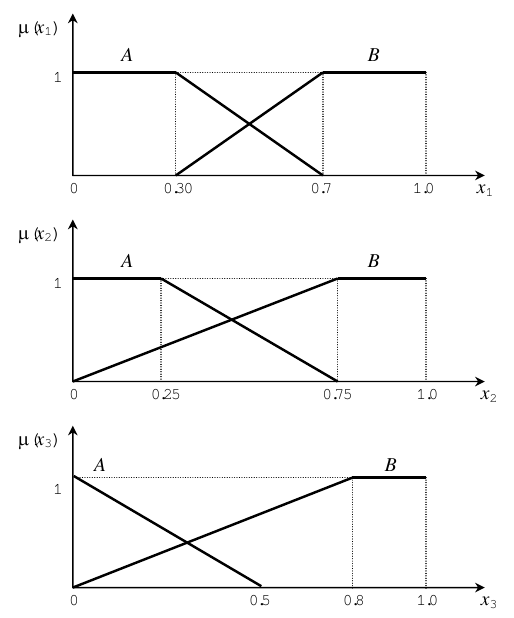
\includegraphics[scale=0.7]{fig.png}
\caption{Funções de pertinência das variáveis de entrada.}
\label{fig:fig1}
\end{figure}

Sabendo-se que todas as possíveis regras $R_i$ são do tipo ''Se ($x_1$ é ...) e ($x_2$ é ...) e ($x_3$ é ...)
Então $f_i(x_1, x_2, x_3)$'', faça as seguintes atividades:

\begin{enumerate}
\item[1.] Obtenha as funções de regressão $f_i$ associadas a cada uma das possíveis regras, avaliando-se
também se cada uma delas representa com fidelidade a respectiva aproximação realizada.\\
Regra 1:Valores[d a b c] para f=a*x1+b*x2+c*x3+d: [ 0.04059265  0.43720663  0.42461106  0.46301813] \\
Regra 2:Valores[d a b c] para f=a*x1+b*x2+c*x3+d: [ 0.07886731  0.4247315   0.42374505  0.3350464 ] \\
Regra 3:Valores[d a b c] para f=a*x1+b*x2+c*x3+d: [ 0.06671982  0.44056935  0.33137225  0.4631357 ] \\
Regra 4:Valores[d a b c] para f=a*x1+b*x2+c*x3+d: [ 0.09422252  0.4356258   0.34008417  0.34640704] \\
Regra 5:Valores[d a b c] para f=a*x1+b*x2+c*x3+d: [ 0.13388251  0.2474547   0.42442706  0.47046929] \\
Regra 6:Valores[d a b c] para f=a*x1+b*x2+c*x3+d: [ 0.1493849   0.27159103  0.43799894  0.33341693] \\
Regra 7:Valores[d a b c] para f=a*x1+b*x2+c*x3+d: [ 0.14439789  0.26989667  0.33911343  0.45950501] \\
Regra 8:Valores[d a b c] para f=a*x1+b*x2+c*x3+d: [ 0.17017642  0.27434641  0.35449356  0.33468562] \\

\item[2.] Elabore os procedimentos computacionais necessários para obter os valores de saída do
método de Takagi-Sugeno em função das contribuições resultantes de todas as regras
ativadas.\\
Os procedimentos estão no código anexado.

\item[3.] Considere os seguintes valores de $x_1, x_2 e x_3$ que foram adquiridos em tempo real pelos
instrumentos de medição do processo, os quais são definidos por:

As regras $R_i$ são do tipo ''Se ($x_1$ é ...) e ($x_2$ é ...) e ($x_3$ é ...)
Então $f_i(x_1, x_2, x_3)$'', estão listadas na tabela abaixo:\\

\begin{center}
\begin{tabular}{ll}
Regra & Funções ativas(x1:x2:x3)\\
Regra 1 & AAA\\
Regra 2 & AAB\\
Regra 3 & ABA\\
Regra 4 & ABB\\
Regra 5 & BAA\\
Regra 6 & BAB\\
Regra 7 & BBA\\
Regra 8 & BBB
\end{tabular}
\end{center}

\begin{enumerate}
\item[a)] Valor de $x_1$ = 0,1399 e $x_2$ = 0,1610 e $x_3$ = 0,2477\\
Regra 1 , y da regra: 0.284809830064 peso da regra 0.505505505506 \\
Regra 2 , y da regra: 0.289501198838 peso da regra 0.309059059059 \\
Regra 3 , y da regra: 0.296425119576 peso da regra 0.214881548215 \\
Regra 4 , y da regra: 0.295725149287 peso da regra 0.214881548215 \\
Resposta y= 0.289865831231

\item[b)]Valor de $x_1$ = 0,9430 e $x_2$ = 0,4476 e $x_3$ = 0,2648\\
Regra 5 , y da regra: 0.681786107175 peso da regra 0.471471471471 \\
Regra 6 , y da regra: 0.689832367726 peso da regra 0.33033033033 \\
Regra 7 , y da regra: 0.672374545124 peso da regra 0.471471471471 \\
Regra 8 , y da regra: 0.676181160042 peso da regra 0.33033033033 \\
Resposta y= 0.67952192971

\item[c)]Valor de $x_1$ = 0,0004 e $x_2$ = 0,6916 e $x_3$ = 0,5006\\
Regra 2 , y da regra: 0.539823513565 peso da regra 0.116616616617 \\
Regra 4 , y da regra: 0.50301035033 peso da regra 0.625625625626 \\
Resposta y= 0.508794212119

\item[d)]Valor de $x_1$ = 0,5102 e $x_2$ = 0,7464 e $x_3$ = 0,0860\\
Regra 1 , y da regra: 0.620404723659 peso da regra 0.00650650650651 \\
Regra 2 , y da regra: 0.640662621487 peso da regra 0.00650650650651 \\
Regra 3 , y da regra: 0.578664224572 peso da regra 0.473723723724 \\
Regra 4 , y da regra: 0.600108637446 peso da regra 0.107607607608 \\
Regra 5 , y da regra: 0.617386611231 peso da regra 0.00650650650651 \\
Regra 6 , y da regra: 0.643546906933 peso da regra 0.00650650650651 \\
Regra 7 , y da regra: 0.574730861855 peso da regra 0.526276276276 \\
Regra 8 , y da regra: 0.603524919873 peso da regra 0.107607607608 \\
Resposta y= 0.582097748324

\item[e)]Valor de $x_1$ = 0,0611 e $x_2$ = 0,2860 e $x_3$ = 0,7464\\
Regra 2 , y da regra: 0.476088129606 peso da regra 0.927427427427 \\
Regra 4 , y da regra: 0.476661549281 peso da regra 0.381715048382 \\
Resposta y= 0.47625532525

\end{enumerate}
Determine, para cada um dos valores acima, o valor final de saída do sistema \emph{fuzzy}
considerando a contribuição de cada uma das regras ativadas e suas respectivas funções de
regressão, listando ainda quais as regras \emph{fuzzy} que estarão associadas com o cálculo do
resultado final do sistema \emph{fuzzy}.
\end{enumerate}


\newpage
\lstset{basicstyle=\footnotesize}
\lstinputlisting[language=Python]{epc8.py}

\end{document}
